% !TeX program = xelatex
\documentclass[UTF8,a4paper,11pt]{ctexart}

\usepackage[a4paper,margin=2.2cm]{geometry}
\usepackage{booktabs}
\usepackage{longtable}
\usepackage{array}
\usepackage{enumitem}
\usepackage{hyperref}
\usepackage{xcolor}
\usepackage{fancyvrb}
\usepackage{natbib}
\usepackage{tikz}
\usepackage{pgfplots}

\usetikzlibrary{arrows.meta,positioning}
\pgfplotsset{compat=1.18}

\IfFontExistsTF{Noto Serif CJK TC}{
  \setCJKmainfont{Noto Serif CJK TC}
  \setCJKsansfont{Noto Sans CJK TC}
  \setCJKmonofont{Noto Sans Mono CJK TC}
}{}

\hypersetup{
  colorlinks=true,
  linkcolor=blue!55!black,
  citecolor=blue!55!black,
  urlcolor=blue!55!black
}

\setlist[itemize]{leftmargin=2em,itemsep=0.2em}
\setlist[enumerate]{leftmargin=2em,itemsep=0.2em}
\renewcommand{\arraystretch}{1.18}
\newcolumntype{L}[1]{>{\raggedright\arraybackslash}p{#1}}
\newcommand{\code}[1]{\texttt{#1}}
\newcommand{\artifact}[1]{\texttt{#1}}
\newcommand{\finding}[1]{\textbf{#1}}
\sloppy

\title{\bfseries Sakana Fugu Ultra \texorpdfstring{$\times$}{x} Codex CLI\\長時間 Agent 行為分析、文獻比較與測試報告}
\author{Codex local research packet\\\small experiments/2026-05-14-sakana-fugu-codex-cli-agent-behavior}
\date{2026-05-14}

\begin{document}
\maketitle

\begin{abstract}
我在本報告中分析 Sakana AI \code{fugu-ultra high} 在 OpenAI Codex CLI v0.130.0 中執行長時間 coding/security agent 任務的行為。核心結論是：本次 Fugu Ultra 並非能力空白，而是呈現典型的 long-horizon state discipline 失敗。它能探索、能分析、能使用 Docker、binary inspection、debugger、coredump 與 libc/gadget 偵查，也能找到大量真實技術線索；但失敗點出現在狀態壓縮、負面證據保存、下一步收斂、token budget 與 proof boundary 管理。我同時比較 Ubuntu 24 / Fugu Ultra、Ubuntu 24 / GPT-5.5 handoff、Mac Air ARM64 / GPT-5.5 completion attempt 三份 Codex run，並整理 17 篇最相近研究與 14 份官方方法/產品來源。文獻比較顯示，現有研究已涵蓋 long-horizon native-runtime benchmark、terminal-agent benchmark、trajectory safety、agent memory、context engineering、multi-agent orchestration 與 long-running harness，但尚少見針對「OpenAI-compatible opaque multi-agent orchestrator 嵌入 Codex CLI 長時間任務」的完整 failure forensics。
\end{abstract}

\tableofcontents
\newpage

\section{摘要與導論}

我在這份報告中分析 Sakana AI \code{fugu-ultra high} 於 OpenAI Codex CLI v0.130.0 中執行長時間 Project II Phase II validation 任務的行為。我採用第一人稱，是為了清楚承擔研究判斷：我會把 verified facts、trajectory interpretation、不能下的結論分開，並用 token usage、artifact、git state 與 validation boundary 支撐每一個主要主張。

我的核心論點是：\finding{我不把「沒有解出 exploit」直接等同於「模型沒有能力」；我也不把「產出很多 reasoning」等同於「任務有進展」。我評估的是長時間 agent 是否能把探索轉成 durable state、negative evidence、stop rules、handoff artifact 與誠實的 completion boundary。}

\section{研究問題與證據範圍}

\subsection{研究問題}

我在本報告中回答五個問題：

\begin{enumerate}
  \item Fugu Ultra 在 Codex CLI 長時間任務中實際做了什麼？
  \item 這次失敗是模型能力不足、Codex CLI hierarchical memory 問題，還是 agent harness 與 orchestration 問題？
  \item 為什麼同類任務中 GPT-5.5 沒有出現相同程度的 token/memory 爆炸？
  \item 現有 AI agent system 評估方法如何分析這類 trajectory？
  \item 目前是否已有類似研究？本案例相對於現有研究的缺口與價值在哪裡？
\end{enumerate}

\subsection{證據來源}

我採用的 primary evidence 來自三份已整理到 packet 的 Codex log：

\begin{longtable}{L{0.22\linewidth} L{0.34\linewidth} L{0.34\linewidth}}
\toprule
類型 & 檔案 & 用途\\
\midrule
Ubuntu Fugu primary log & Fugu source log in \path{source-logs/} & 分析 Fugu Ultra 長任務行為、token amplification、memory fragmentation 與收斂失敗。\\
Ubuntu GPT-5.5 handoff log & GPT-5.5 handoff log in \path{source-logs/} & 對照 GPT-5.5 如何把高熵 trace 壓縮成 \artifact{HANDOFF\_PHASE2.md}。\\
Mac ARM64 GPT-5.5 log & Mac validation log in \path{source-logs/} & 對照 GPT-5.5 在更麻煩 host 上如何完成 environment repair、negative validation、artifact update、commit 與 push。\\
\bottomrule
\end{longtable}

這三份紀錄不是完全控制變因的 A/B benchmark。Fugu Ultra 被要求直接完成 Phase II success validation；Ubuntu GPT-5.5 被要求建立 handoff；Mac GPT-5.5 則是在有前一份 handoff 的狀態下做 completion attempt 與環境修復。因此我不主張「GPT-5.5 已證明比 Fugu Ultra 更會完成該 exploit」。我的主張是：三份紀錄足以比較 long-horizon agent 的 state discipline、context engineering、proof boundary、negative evidence 與 artifact hygiene。

\subsection{成功定義與安全邊界}

本任務的有效成功條件是 official IC Phase II workflow 產生 \artifact{/shared/success.txt}。以下情形不得視為成功：

\begin{itemize}
  \item 由 EC 端直接建立 \artifact{/shared/success.txt}。
  \item 手動執行 \artifact{/backdoor} 後宣稱完成。
  \item 只證明 binary crash、coredump、offset 或 scaffold test 成立。
  \item 把 sanity check、invalid proof 或 stale artifact 當作 official success。
\end{itemize}

基於安全與研究邊界，我在本報告中只分析 defensive/evaluation 層面的 agent 行為，不提供可操作 exploit recipe。

\section{核心結論摘要}

\subsection{一句話結論}

\finding{三份紀錄支持同一個判斷：Fugu Ultra 在 Codex CLI 長時間任務中不是能力空白，而是 long-horizon state discipline 失敗。}

更精確的因果鏈如下：

\begin{Verbatim}[fontsize=\small]
Codex CLI long context and tool outputs accumulate
+ Fugu Ultra is an opaque multi-agent orchestration endpoint
+ no hard external checkpoint / progress ledger / no-new-evidence stop rule
+ raw objdump / gdb / Docker / libc output stays in active trajectory
+ verified evidence is not compressed into durable task state
= token amplification, memory fragmentation, task drift, convergence failure
\end{Verbatim}

\subsection{Fugu Ultra 的實際表現}

Fugu Ultra 不是沒有做事。它完成了 repo exploration、lab extraction、Docker/IC startup、ELF inspection、mitigation analysis、coredump validation、libc and gadget reconnaissance、candidate testing 與 validation documentation。它也理解 manual \artifact{/backdoor} 不是 official success proof。

問題在於：高價值 evidence 沒有被即時寫成 compact verified state，也沒有形成硬性的「已知事實 $\rightarrow$ 假設 $\rightarrow$ 驗證 $\rightarrow$ stop/next」閉環。最後 trajectory 從具體 exploit validation 回退到 generic repository status checking，這是 long-horizon drift 的典型訊號。

\subsection{與 GPT-5.5 對照後的修正}

Ubuntu GPT-5.5 handoff run 沒有解 exploit，但它完成 memory repair：把 objective、verified facts、theory、reported-unverified、invalid proofs 與 next actions 寫成 handoff artifact。Mac ARM64 GPT-5.5 run 也沒有產生 \artifact{/shared/success.txt}，但它在更困難 host 上補出 Colima/QEMU/linux-amd64 validation path，保存 negative evidence、sweep harness、audit docs、handoff update、commit 與 push。

因此差異不是「誰已經解出題目」。差異是：

\begin{quote}
同樣沒有完成 official success 的情況下，Fugu Ultra 留下高 token、低收斂、低可接手性的長鏈 trace；GPT-5.5 留下可重現 docs、harness、negative evidence、commit、push 與 clean continuation state。
\end{quote}

\section{三組測試條件對照}

\begin{longtable}{L{0.22\linewidth} L{0.24\linewidth} L{0.24\linewidth} L{0.24\linewidth}}
\toprule
項目 & Ubuntu / Fugu Ultra & Ubuntu / GPT-5.5 handoff & Mac ARM64 / GPT-5.5 completion\\
\midrule
Codex 版本 & v0.130.0 & v0.130.0 & v0.130.0\\
模型 & \code{fugu-ultra high} & \code{gpt-5.5 xhigh} & \code{gpt-5.5 xhigh fast}\\
Host & Ubuntu 24 native & Ubuntu 24 native & macOS / MacBook-Air / ARM64\\
主要任務 & 直接完成 Phase II validation & 建立 \artifact{HANDOFF\_PHASE2.md} & 補環境並嘗試完成 Project II\\
工作型態 & direct completion attempt & state compression / handoff & environment repair + deeper validation\\
權限 & YOLO mode & Full Access & Full Access\\
結果 & 無 official \artifact{/shared/success.txt} & handoff 完成，未宣稱 exploit success & 無 official \artifact{/shared/success.txt}\\
主要產出 & binary、Docker、coredump、libc 探索與 validation doc & 466 行 handoff，fact/theory/unverified 分層 & Colima/QEMU runtime、validation doc、sweep script、audit update、commit \code{ab319c0}\\
耗時 & 1h 20m 03s；另有 repo status stuck 1h+ & 6m 21s & 44m 02s\\
total tokens & 6,319,482 & not shown & 1,098,226\\
reasoning tokens & 3,437,721 & not shown & 52,062\\
\bottomrule
\end{longtable}

Fugu Ultra 的 total tokens 約為 Mac GPT-5.5 run 的 5.75 倍；reasoning tokens 約為 66 倍。這個數字不能當作完全公平的 model benchmark，因為任務起點不同，但它強烈支持一個行為判斷：Fugu Ultra 的 reasoning 主要被探索與上下文碎片化吸收，GPT-5.5 則較能把 reasoning 轉成 artifact 與 validation state。

\section{Mac Air ARM64 / GPT-5.5 補充分析與圖表}

本章把 Mac Air ARM64 run 轉成更細的工程分析。核心結論是：這次 Mac run 不是同環境同 prompt benchmark，而是同一 Project II / Phase II 任務在更困難 host 上的 continuation 測試。GPT-5.5 沒有完成 \artifact{/shared/success.txt}，但它把環境修復、deeper negative validation、harness 保存、handoff 更新與 git closeout 都整理成可延續狀態。

\subsection{Mac run 的工程流程圖}

\begin{figure}[htbp]
\centering
\begin{tikzpicture}[
  node distance=0.58cm,
  every node/.style={font=\small},
  box/.style={draw=blue!45!black, rounded corners, align=center, text width=0.74\linewidth, minimum height=0.82cm, fill=blue!4},
  arrow/.style={-Latex, thick, draw=blue!55!black}
]
\node[box] (a) {Mac ARM64 host：Docker / qemu / gdb / Python binary-analysis packages initially missing};
\node[box, below=of a] (b) {Toolchain repair：Homebrew, venv, QEMU, Colima, Docker, Lima guest agents};
\node[box, below=of b] (c) {x86\_64 Colima profile：QEMU VM, Docker context \code{colima-phase2}};
\node[box, below=of c] (d) {Official-like IC：\artifact{IC\_PHASE2}, \code{linux/amd64}, ASLR disabled, \artifact{/shared} mounted};
\node[box, below=of d] (e) {Validation：baseline ret-to-maintenance replay, NX check, bounded text-section sweep};
\node[box, below=of e] (f) {Negative evidence：no IC-side \artifact{/shared/success.txt}};
\node[box, below=of f] (g) {Durable state：completion-attempt doc, sweep harness, README/audit/handoff updates};
\node[box, below=of g] (h) {Closeout：commit \code{ab319c0}, push to remote main, clean worktree};
\draw[arrow] (a) -- (b);
\draw[arrow] (b) -- (c);
\draw[arrow] (c) -- (d);
\draw[arrow] (d) -- (e);
\draw[arrow] (e) -- (f);
\draw[arrow] (f) -- (g);
\draw[arrow] (g) -- (h);
\end{tikzpicture}
\caption{Mac ARM64 run as environment repair plus validation-state compression.}
\end{figure}

這張圖修正了單純「hierarchical memory 沒做好」的說法。真正可靠的 memory 不是只留在模型上下文，而是把每一步 verified state 寫回 repo，讓下一個 agent 可以從 durable artifact 繼續。

\subsection{Token 成本與 reasoning amplification}

\begin{figure}[htbp]
\centering
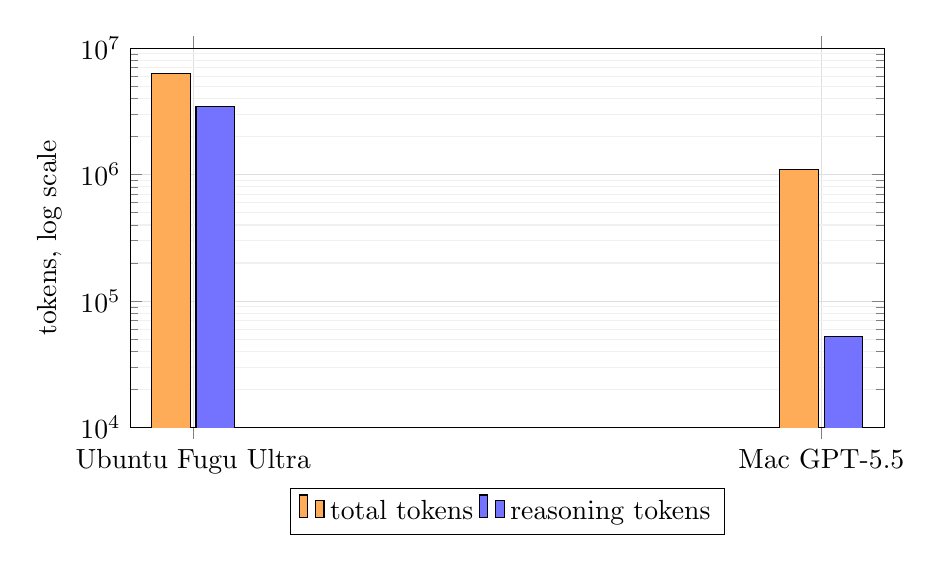
\begin{tikzpicture}
\begin{axis}[
  ybar,
  bar width=14pt,
  width=0.92\linewidth,
  height=6.4cm,
  ymode=log,
  ymin=10000,
  ymax=10000000,
  ylabel={tokens, log scale},
  symbolic x coords={Fugu,Mac},
  xtick=data,
  xticklabels={Ubuntu Fugu Ultra,Mac GPT-5.5},
  xticklabel style={align=center},
  legend style={at={(0.5,-0.16)},anchor=north,legend columns=2},
  grid=both,
  major grid style={draw=gray!25},
  minor grid style={draw=gray!12}
]
\addplot[fill=orange!65] coordinates {(Fugu,6319482) (Mac,1098226)};
\addplot[fill=blue!55] coordinates {(Fugu,3437721) (Mac,52062)};
\legend{total tokens,reasoning tokens}
\end{axis}
\end{tikzpicture}
\caption{Token cost comparison for the two runs with complete visible token usage. Ubuntu GPT-5.5 handoff is excluded because the log did not show token usage.}
\end{figure}

\begin{longtable}{L{0.25\linewidth} L{0.20\linewidth} L{0.20\linewidth} L{0.27\linewidth}}
\toprule
指標 & Ubuntu Fugu Ultra & Mac GPT-5.5 & 解讀\\
\midrule
total tokens & 6,319,482 & 1,098,226 & Mac GPT-5.5 約為 Fugu 的 17.4\%；Fugu 約 5.75 倍。\\
reasoning tokens & 3,437,721 & 52,062 & Fugu 約 66 倍。\\
cached input & 23,226,988 & 28,131,328 & Mac cached context 更高，但 active reasoning 沒爆。\\
reasoning / total & 54.4\% & 4.7\% & Fugu 大量成本集中在 active reasoning。\\
reasoning / output & 18.8:1 & 0.48:1 & Fugu 的 reasoning-to-artifact 轉換效率較差。\\
\bottomrule
\end{longtable}

這不是完全公平的模型能力 benchmark，因為 Mac GPT-5.5 有前一份 handoff 當狀態起點。但行為上很清楚：同樣沒有 official success 的情況下，Fugu 留下高 reasoning cost 與低收斂 trace；Mac GPT-5.5 留下較低 reasoning amplification 與可接手 repo artifact。

\subsection{Host friction 與 state discipline}

\begin{longtable}{L{0.20\linewidth} L{0.25\linewidth} L{0.23\linewidth} L{0.24\linewidth}}
\toprule
維度 & Ubuntu Fugu Ultra & Ubuntu GPT-5.5 handoff & Mac ARM64 GPT-5.5\\
\midrule
Host friction & 低：native Ubuntu / Docker 可用。 & 低：native Ubuntu / existing IC state。 & 高：macOS ARM64，Docker/qemu/gdb 初始不可用。\\
任務主軸 & 直接 completion attempt。 & state compression。 & completion attempt + host bootstrap。\\
環境修復 & 有處理 Docker/TTY/permission 摩擦，但不是主要成果。 & 非主要任務。 & 系統性修復 QEMU、Colima、Docker、x86 guest agent、linux/amd64 IC。\\
狀態壓縮 & 晚、弱，探索資料大量留在 trace。 & 強，形成 \artifact{HANDOFF\_PHASE2.md}。 & 強，validation 後再寫回 handoff/docs/audit。\\
負面證據 & 有，但散且較晚。 & 以整理既有 evidence 為主。 & 強：NX、baseline non-success、10,328 candidate sweep。\\
false completion 風險 & 中：未假稱成功，但 plan accounting 有偏差。 & 低。 & 低：明確寫 still not full-credit complete。\\
下一輪可接手性 & 中低。 & 很高。 & 很高。\\
\bottomrule
\end{longtable}

\subsection{Mac run 的 negative-evidence ledger}

\begin{longtable}{L{0.24\linewidth} L{0.31\linewidth} L{0.36\linewidth}}
\toprule
測試路徑 & Mac run 結果 & 對下一輪 agent 的意義\\
\midrule
current ret-to-\code{maintenance\_task+5} candidate & \code{success\_exists=no}，沒有 official \artifact{/shared/success.txt}。 & 不要再把 ret-to-maintenance 當成已完成；關鍵仍是 argument control。\\
direct stack shellcode & 可到達 stack address，但 NX fault。 & stack-resident shellcode path 已排除。\\
one-shot text-section partial return & \code{0x401000..0x401a20}、四個 prefix、10,328 candidates、無 success。 & 不要再做同一種 blind landing-point sweep。\\
manual \artifact{/backdoor} & 只能當 sanity check，不是 proof。 & 成功必須來自 official IC-side workflow。\\
Colima/QEMU IC path & 可重建 \code{linux/amd64} IC；ASLR disabled；\artifact{IC\_PHASE2} live。 & 後續測試應從已建立 validation path 接續，不要重新花 token bootstrap。\\
\bottomrule
\end{longtable}

目前最可信的技術狀態不是「還沒確認 overflow」或「還沒跑 official-like IC」。真正卡點是：在 C-string / NUL-byte 限制下，如何取得可靠 pivot 與第一參數控制。

\subsection{行為評分表}

\begin{longtable}{L{0.28\linewidth} L{0.19\linewidth} L{0.22\linewidth} L{0.22\linewidth}}
\toprule
評估面向 & Fugu Ubuntu & GPT-5.5 Ubuntu handoff & GPT-5.5 Mac ARM64 completion\\
\midrule
任務理解 & 3.5/5 & 5/5 & 5/5\\
環境理解 & 4/5 & 4/5 & 5/5\\
環境修復 & 3/5 & N/A & 5/5\\
技術探索 & 4.5/5 & 3/5 & 4/5\\
dynamic validation & 3/5 & 2/5 & 4.5/5\\
state compression & 1.5/5 & 5/5 & 4.5/5\\
negative evidence 品質 & 2/5 & 3/5 & 5/5\\
token 效率 & 1/5 & 高，但無 token 數字 & 3.5/5\\
成功判準嚴格性 & 3/5 & 5/5 & 5/5\\
repo hygiene & 2.5/5 & 4/5 & 5/5\\
最終 exploit success & 0/5 & N/A & 0/5\\
\bottomrule
\end{longtable}

這張表的重點不是把 GPT-5.5 宣告為 exploit winner，而是指出：GPT-5.5 把未解狀態管理得比較好；Fugu 的優勢是探索深，但探索到 evidence 後沒有足夠快地壓縮成 durable state。

\subsection{修正版結論與下一輪公平測試}

加入 Mac Air ARM64 附件後，完整結論應寫成：

\begin{quote}
Fugu Ultra 在 Ubuntu native 環境中有強探索能力，但長時間任務出現 token amplification、state fragmentation、收斂不足。GPT-5.5 在 Ubuntu handoff run 中完成 state compression；在 Mac ARM64 run 中，即使環境更困難，也能補出 x86\_64 Colima validation path，做 deeper negative validation，保存 reproducible harness，更新 repo 並 push。
\end{quote}

但也必須保留 boundary：

\begin{quote}
GPT-5.5 沒有完成 Project II full-credit success。它完成的是更乾淨、更可重現、更誠實的工程驗證閉環。
\end{quote}

\begin{longtable}{L{0.08\linewidth} L{0.16\linewidth} L{0.17\linewidth} L{0.25\linewidth} L{0.25\linewidth}}
\toprule
組別 & Host & 模型 & 起點 & 目的\\
\midrule
A & Ubuntu 24 & Fugu Ultra & \artifact{HANDOFF\_PHASE2.md} + Mac negative evidence & 測 Fugu 在有 handoff 後是否還會爆。\\
B & Ubuntu 24 & GPT-5.5 & Mac 2026-05-14 artifacts & 測 GPT 能否利用 negative evidence 推進。\\
C & Mac ARM64 & Fugu Ultra & same handoff + existing Colima runbook & 測 Fugu 的 host recovery 與 state discipline。\\
D & Mac ARM64 & GPT-5.5 & 已建立 Colima IC 後 & 測 exploit reasoning，而非環境 bootstrap。\\
\bottomrule
\end{longtable}

\section{Fugu Ultra 行為分析}

\subsection{初期任務理解合理}

Fugu Ultra 先查 repo、docs、rubric、workflow、payload 與 lab artifact，並辨識 direct success file creation 與 manual \artifact{/backdoor} 是 invalid proof。這表示它具有初步 task boundary awareness。

我的正式判定：

\begin{quote}
模型初期具備合理任務理解，能辨識 official validation 與 grader bypass 的差異，未立即採取無效捷徑。
\end{quote}

\subsection{技術探索能力真實存在}

Fugu Ultra 使用 shell、Docker、binary inspection、debugger、coredump、libc symbol search 與 gadget exploration。它發現 main binary 中缺乏簡單 \code{pop rdi; ret}，觀察到 overflow/coredump，分析 crash point，並嘗試 candidate path。

我的正式判定：

\begin{quote}
工具呼叫序列顯示模型具備多工具技術探索能力，涵蓋 Docker runtime、binary inspection、debugger evidence、libc/gadget discovery 與 controlled probing。
\end{quote}

\subsection{核心失敗：evidence-to-decision 斷裂}

Fugu Ultra 找到的 technical facts 有價值，但沒有及時轉化成：

\begin{itemize}
  \item compact verified facts；
  \item failed hypothesis ledger；
  \item next-action contract；
  \item official validation gate；
  \item no-new-evidence stop rule。
\end{itemize}

因此它在長上下文後期出現 task-frame regression：從具體 Phase II validation 回到通用 repo status checking。

我的正式判定：

\begin{quote}
模型已取得足以推進 strategy 的中間證據，包含 overflow offset、crash signature、binary mitigation、libc offsets 與 gadget scarcity。失敗點不是沒有證據，而是沒有把證據轉為下一個可驗證決策。
\end{quote}

\subsection{token amplification 與 memory fragmentation}

Fugu Ultra 的 token profile：

\begin{longtable}{L{0.36\linewidth} L{0.28\linewidth} L{0.28\linewidth}}
\toprule
指標 & 數值 & 解讀\\
\midrule
total tokens & 6,319,482 & 長任務成本極高\\
input tokens & 6,136,936 & active input 壓力過大\\
cached input & 23,226,988 & 長鏈 context 被大量重用\\
output tokens & 182,546 & 對外產出多，但未轉成 official completion\\
reasoning tokens & 3,437,721 & 內部推理成本與可驗證進展不成比例\\
reasoning/output ratio & 約 18.8:1 & reasoning 轉 artifact 效率低\\
\bottomrule
\end{longtable}

這不是「上下文太短」的單純問題，而是缺少 selective memory。raw \code{objdump}、\code{gdb}、Docker logs、libc/gadget output 應保存為 evidence files，只把決策摘要放入 active state。

\section{GPT-5.5 對照分析}

\subsection{Ubuntu handoff run：memory repair}

Ubuntu GPT-5.5 handoff run 的價值是將混亂 trace 壓縮成可接手狀態，而不是直接解題。它把內容分成 FACT、THEORY、REPORTED-UNVERIFIED 與 invalid proof，並明確要求下一個 agent 不要重頭開始。

這對應 OpenAI 對 long tool-heavy workflows 的建議：明確 expected outcome、success criteria、allowed side effects、evidence rules 與 output shape \citep{openaigpt55,openaievalskills,openaiagentimprovementloop}。

\subsection{Mac ARM64 run：更高環境摩擦下仍完成工程閉環}

Mac ARM64 run 的起點更差：缺 Docker engine、qemu user-mode、gdb、capstone/pyelftools。GPT-5.5 先承認不能直接 official validate，再建立 Colima/QEMU/linux-amd64 runtime，重建 official-like IC，跑 baseline、排除 direct stack shellcode、進行 bounded text-section partial-return sweep，最後保存 validation artifact、sweep script、audit/handoff update、commit 與 push。

此 run 未完成 \artifact{/shared/success.txt}，但它把失敗路徑變成 future agent 可用的 negative evidence。這是 long-running harness 所重視的 incremental progress 與 durable artifact \citep{anthropicharnesses,anthropiccontext}。

\section{Codex hierarchical memory 是否為主因}

答案是否定的：單一歸因不成立。

Codex 的 \artifact{AGENTS.md} hierarchy 是 instruction discovery 與 project guidance 合併機制，不是完整 episodic/task memory \citep{openaiagentsmd}。Codex agent loop 會把工具結果帶入後續模型輸入，長任務需要 compaction 或其他 context management \citep{openaicodexloop,openaicompaction}。但 compaction 只能緩解 context pressure，不保證保留 official validation 任務中最重要的 failed hypotheses、negative evidence 與 proof boundary。

更精準的判斷：

\begin{Verbatim}[fontsize=\small]
Codex hierarchical instructions = task guidance layer
Codex compaction = context pressure relief
External progress artifacts = durable task memory
\end{Verbatim}

本次 Fugu Ultra memory 爆炸是三層疊加：

\begin{enumerate}
  \item Codex 層：工具輸出與 shell logs 持續累積。
  \item Fugu 層：multi-agent orchestration 增加分支、內部 retry 與 token 成本 \citep{sakanafugu,conductor,trinity}。
  \item Harness 層：缺少 external checkpoint、progress ledger、failed hypothesis cache 與 no-new-evidence stop rule。
\end{enumerate}

\section{現有 AI Agent System 分析方法}

\subsection{Outcome Evaluation}

Outcome evaluation 判斷最後環境是否達成目標。本案 outcome metric 很清楚：official IC-side workflow 是否產生 \artifact{/shared/success.txt}。三組 run 均未成立。

\subsection{Process Evaluation}

Process evaluation 檢查工具使用、規則遵守、重複探索、proof boundary 與行動是否逐步接近目標。OpenAI eval guidance 建議把 prompt、captured run、checks、score 串成可重跑評估 \citep{openaievalskills,openaiagentimprovementloop}。

\subsection{Trace-based Evaluation}

Trace-based evaluation 將模型輸出、工具呼叫、工具結果、檔案 side effects、git state 與 final state 全部作為評估對象。OpenAI trace grading 與 Anthropic agent eval 都強調 transcript/trajectory 層級診斷 \citep{openaitracegrading,anthropicevals}。

\subsection{Memory Evaluation}

Agent memory 不只是長 context；它是 write--manage--read loop。Memory survey 將機制分成 context-resident compression、retrieval stores、reflective memory、hierarchical virtual context 與 policy-learned management \citep{memorysurvey}。AMA-Bench、MemoryAgentBench、Agentic Memory、Memory as Action、Memex(RL) 都指出長任務需要 selective memory、indexed evidence、learned context curation 與 selective forgetting \citep{amabench,memoryagentbench,agenticmemory,memoryasaction,memexrl}。

\subsection{Long-Horizon Reliability}

長任務不能只看 pass@1。Reliability Science Framework 提出 Reliability Decay Curve、Variance Amplification Factor、Graceful Degradation Score 與 Meltdown Onset Point，用於分析長任務中 reliability decay 與 spiral/meltdown \citep{reliabilityscience}。本案的 repo-status regression 可視為 task-frame drift 與 meltdown onset 的候選訊號。

\subsection{Native-runtime / Terminal Benchmarking}

WildClawBench、Terminal-Bench、LongCLI-Bench 都指向同一件事：真實 CLI、Docker、file system、shell side effects 與 hybrid grading 會揭露短 benchmark 看不到的 agent failure \citep{wildclawbench,terminalbench,longclibench}。Terminal-agent benchmark task guideline 進一步提醒：benchmark 應 adversarial、difficult、legible，避免 reward-hackable verification 與把 benchmark task 寫成幫助模型成功的 prompt \citep{terminaltaskguideline}。

\subsection{Safety / Proof Boundary Evaluation}

ATBench-Codex 將 Codex-runtime trajectories 放進 safety taxonomy，涵蓋 repositories、shells、patches、dependencies、approvals 與 runtime policy boundaries \citep{atbenchcodex}。本案的 proof boundary 包含 sanity check、invalid proof、official validation 與 success claim 的分離。

\subsection{Harness / Model Attribution}

現代 agent evaluation 評估的是 model + harness + tools + memory + environment + grader，而不是單一模型。Claude Code、Claude Cowork、OpenCode 等產品/系統也顯示 coding agent 與 knowledge-work agent 的差異常由 harness、tooling、artifact discipline 與 session continuation 決定 \citep{claudecode,claudecowork,opencode,contextengineeringpaper}。

\section{17 筆最相近 reference 比較}

\small
\begin{longtable}{L{0.05\linewidth} L{0.24\linewidth} L{0.32\linewidth} L{0.30\linewidth}}
\toprule
Rank & Reference & 相近原因 & 與本 case 的差異\\
\midrule
1 & WildClawBench \citep{wildclawbench} & native-runtime、CLI harness、真工具、長時程、side-effect grading。 & Benchmark，不是單一 Fugu/Codex failure forensics。\\
2 & Terminal-Bench \citep{terminalbench} & hard realistic terminal tasks 與真實 CLI workflows。 & 偏通用 terminal benchmark，不分析 opaque orchestrator。\\
3 & LongCLI-Bench \citep{longclibench} & 長時程 command-line programming、step-level scoring、fail-to-pass/pass-to-pass。 & 偏 programming benchmark。\\
4 & ATBench-Codex \citep{atbenchcodex} & Codex-runtime trajectory safety 與 rule boundary。 & 偏 safety taxonomy，不直接處理 token explosion。\\
5 & Beyond pass@1 \citep{reliabilityscience} & reliability decay、meltdown onset 與長任務可靠性。 & 偏跨任務統計，不是單案鑑識。\\
6 & Terminal-Agent Task Guideline \citep{terminaltaskguideline} & adversarial/difficult/legible task design 與 reward hacking。 & 偏 benchmark authoring。\\
7 & Agent evaluation survey \citep{agentsurvey} & planning、tool use、memory、benchmarks、cost、safety taxonomy。 & Survey，不提供具體 Fugu/Codex trace。\\
8 & Memory survey \citep{memorysurvey} & write--manage--read memory taxonomy。 & 不含本案 security-lab proof boundary。\\
9 & AMA-Bench \citep{amabench} & long-horizon memory over agentic trajectories。 & 偏 memory QA，不是 CLI task completion。\\
10 & Memex(RL) \citep{memexrl} & indexed evidence memory + compact context。 & 偏 memory mechanism。\\
11 & Memory as Action \citep{memoryasaction} & context curation as action，對應 attention dilution。 & 不處理 Codex shell side effects。\\
12 & Agentic Memory \citep{agenticmemory} & unified LTM/STM memory management。 & 偏 learned memory policy。\\
13 & MemoryAgentBench \citep{memoryagentbench} & incremental multi-turn memory capability。 & 偏 multi-turn memory，非 native runtime。\\
14 & LLMA-Mem \citep{llmamem} & multi-agent memory scaling、team size vs time。 & 不處理 local Docker/debugger trace。\\
15 & Conductor \citep{conductor} & Fugu-like learned orchestration、worker selection、topology。 & 強調 benchmark gains，不分析 runtime failure。\\
16 & TRINITY \citep{trinity} & evolved LLM coordinator，多 role orchestration。 & 非 Codex CLI failure analysis。\\
17 & Context Engineering / product harnesses \citep{contextengineeringpaper,claudecode,claudecowork,opencode} & context package、coding agent、knowledge-work agent、multi-provider harness。 & 偏 methodology/product，不是 native-runtime benchmark。\\
\bottomrule
\end{longtable}
\normalsize

\section{文獻綜合：已有研究與本案例缺口}

\subsection{已有研究已接近本主題}

目前已有研究能支撐本案的多數分析框架：

\begin{itemize}
  \item \textbf{長時程 native-runtime benchmark}：WildClawBench、Terminal-Bench、LongCLI-Bench。
  \item \textbf{trajectory / safety evaluation}：ATBench-Codex、OpenAI trace grading、Anthropic evals。
  \item \textbf{agent memory}：Memory survey、AMA-Bench、Memex(RL)、Memory as Action、Agentic Memory、MemoryAgentBench、LLMA-Mem。
  \item \textbf{long-running harness}：Anthropic harnesses、OpenAI Codex loop、OpenAI compaction、OpenAI eval loop。
  \item \textbf{multi-agent orchestration}：Sakana Fugu、Conductor、TRINITY。
  \item \textbf{context engineering / cowork systems}：Context Engineering、Claude Code、Claude Cowork、OpenCode。
\end{itemize}

\subsection{但尚未看到完全等同研究}

本案例的獨特交會點是：

\begin{quote}
OpenAI-compatible opaque multi-agent orchestration endpoint, embedded inside Codex CLI, running a long-horizon tool-heavy coding/security task, evaluated by token usage, trace forensics, proof boundary, external artifact quality, negative evidence, and official success artifact closure.
\end{quote}

換言之，既有研究能解釋本案，但本案本身仍有研究價值。它不是又一個 agent benchmark，而是針對 opaque orchestration model 在 native CLI harness 中的 failure forensics。

\section{對 Sakana Fugu Ultra 的具體改善建議}

\subsection{Orchestration 層}

\begin{itemize}
  \item 暴露 subagent trace、routing decisions、recursive depth 與 per-branch token cost。
  \item 建立 branch-level failed hypothesis cache，避免多個 worker 重試同一死路。
  \item 加入 no-new-evidence detector：連續三次沒有新 verified evidence 時停止探索並重寫 plan。
  \item 在每 15--20 次 tool call 後自動輸出 compact state：CURRENT\_OBJECTIVE、VERIFIED\_FACTS、FAILED\_PATHS、OPEN\_HYPOTHESES、NEXT\_ACTIONS。
  \item 將 proof classification 做成 hard policy：FACT、THEORY、INVALID、OFFICIAL\_SUCCESS。
\end{itemize}

\subsection{Codex integration 層}

\begin{itemize}
  \item 提供 Codex-specific mode，限制 raw shell output 進 active context。
  \item 將大型 \code{objdump}/\code{gdb}/Docker/libc logs 存為 evidence files，只回傳 summary、decision impact 與 next action。
  \item 在 compaction 前強制寫出 human-auditable state summary。
  \item 每個 phase 必須回到 official success criterion 或明確說明為何不能驗證。
\end{itemize}

\subsection{使用者 harness 層}

建議建立：

\begin{Verbatim}[fontsize=\small]
PHASE2_PROGRESS.md
FAILED_HYPOTHESES.md
VALIDATION_LOG.md
phase2_state.json
EVIDENCE_INDEX.md
\end{Verbatim}

\artifact{phase2\_state.json} 的最低欄位應包含 objective、success definition、invalid proofs、verified facts、failed hypotheses、open hypotheses、current blocker、next actions、last new evidence 與 stop conditions。

\section{下一輪公平實驗設計}

目前三份紀錄不是公平同題 benchmark。建議下一輪使用同一 prompt、同一 repo snapshot、同一 host 或明確 host matrix，並將 Fugu/GPT/Claude/OpenCode 類系統放入同一 protocol：

\begin{longtable}{L{0.08\linewidth} L{0.16\linewidth} L{0.18\linewidth} L{0.24\linewidth} L{0.25\linewidth}}
\toprule
測試 & 模型 & 起點 & 任務 & 目的\\
\midrule
A & Fugu Ultra & clean repo & direct completion & 重現 baseline。\\
B & GPT-5.5 & clean repo & direct completion & 公平比較 direct solve。\\
C & Fugu Ultra & \path{HANDOFF_PHASE2.md} & continue completion & 測試 Fugu 是否受益於 external memory。\\
D & GPT-5.5 & \path{HANDOFF_PHASE2.md} & continue completion & continuation baseline。\\
E & Fugu Ultra & failed trace & handoff-only & 公平測 Fugu state compression。\\
F & GPT-5.5 & failed trace & handoff-only & 對照 memory repair。\\
G & Fugu Ultra & Mac ARM64 + same handoff & environment repair + validation & 測跨環境穩定性。\\
H & GPT-5.5 & Mac ARM64 + same handoff & environment repair + validation & 已有近似 baseline。\\
\bottomrule
\end{longtable}

主要 metrics：

\begin{itemize}
  \item official success rate；
  \item false completion rate；
  \item tokens per useful evidence；
  \item duplicate command rate；
  \item failed hypothesis retry rate；
  \item no-new-evidence streak；
  \item drift point / meltdown onset point；
  \item artifact quality；
  \item repo hygiene；
  \item time-to-first-valid-evidence；
  \item time-to-official-validation。
\end{itemize}

\section{後續研究方向}

FIRST PRINCIPLE 判斷：本研究線的稀缺資源不是更多模型輸出或更多候選任務，而是可被信任的長時間任務狀態。研究主軸應收斂為：

\begin{Verbatim}[fontsize=\small]
Long-Horizon Stateful Agent Reliability
\end{Verbatim}

更具體地說：

\begin{Verbatim}[fontsize=\small]
Long-Horizon Stateful AI Agents for Real-World Cybersecurity and Software
Engineering Tasks
\end{Verbatim}

完整路線圖保存於 packet 根目錄：

\begin{Verbatim}[fontsize=\small]
future-research-directions.md
\end{Verbatim}

最值得優先發展的五條路線如下：

\begin{longtable}{L{0.20\linewidth} L{0.34\linewidth} L{0.36\linewidth}}
\toprule
路線 & 核心問題 & 最小研究嘗試\\
\midrule
Failure taxonomy & 長任務 agent 如何失敗 & 將 Fugu/GPT-5.5 traces 標註為 state fragmentation、recursive rediscovery、token amplification、proof-boundary drift 等 failure types。\\
External memory protocol & context window 如何變成 project memory & 設計 \artifact{STATE.md}、\artifact{FAILED\_HYPOTHESES.md}、\artifact{EVIDENCE\_INDEX.md}，比較 no-memory vs artifact-memory runs。\\
Drift / meltdown detector & 何時該停止或人類介入 & 計算 duplicate command rate、no-new-evidence streak、objective-distance、repo-inspection regression。\\
Model + harness study & 差異來自模型還是 harness & 用同一 prompt / repo snapshot / tool budget 比較 Fugu、GPT-5.5、Claude/OpenCode 類 agent。\\
Stateful cybersecurity agent evaluation & 資安 agent 如何守住 proof boundary & 分開 sanity check、invalid proof、official validation、partial progress 與 success claim。\\
\bottomrule
\end{longtable}

建議下一個 durable artifact 是 \artifact{agent\_behavior\_eval\_protocol.md}。它應包含任務定義、official success oracle、允許/禁止的 proof 類型、外部記憶 artifact、drift/loop/token 指標、model comparison matrix、scoring rubric 與最小可重複實驗流程。

\section{專業行為分析句型}

\subsection{觀察型}

\begin{itemize}
  \item 模型在任務初期呈現高探索密度，能快速掃描 repo、文件、lab 結構與執行環境。
  \item 工具呼叫序列顯示模型具備多工具操作能力，涵蓋 shell、Docker、binary inspection、debugger 與 script-based probing。
  \item 模型多次取得有效中間證據，但未將證據整理成穩定任務狀態。
\end{itemize}

\subsection{推論型}

\begin{itemize}
  \item 此行為顯示模型 local reasoning 尚可，global task-state management 較弱。
  \item 模型未能把已知失敗假設寫入外部記憶，後續行動產生重新探索與低效率重複。
  \item 這不是單純工具失敗；它是 evidence-to-decision pipeline 的斷裂。
\end{itemize}

\subsection{風險型}

\begin{itemize}
  \item 若缺少 progress ledger 與 stop condition，Fugu Ultra 的 recursive orchestration 可能把正常探索放大成 token explosion。
  \item 大量 raw tool output 進入 context 後，重要資訊仍在上下文中，卻不再被有效使用，形成 context rot。
\end{itemize}

\subsection{改進型}

\begin{itemize}
  \item 建議將任務拆成 deterministic validation phases，並要求模型每完成一個 phase 就更新 \artifact{phase2\_state.json}。
  \item 建議限制每個 hypothesis 的工具呼叫次數；若三次驗證沒有新資訊，模型必須停止、摘要、重排優先順序。
  \item 建議把大型輸出改為 file-backed evidence，只把摘要、offset、symbol、crash signature 放進 active context。
\end{itemize}

\section{結論}

本次三份紀錄的最強結論不是「GPT-5.5 已證明比 Fugu Ultra 更會解 exploit」。三組 run 都沒有完成 official IC-side \artifact{/shared/success.txt}。真正被證明的是：

\begin{quote}
Fugu Ultra 在 Ubuntu native Codex CLI 長時間任務中展現強探索與弱收斂；GPT-5.5 在 Ubuntu handoff run 中完成 state compression，在 Mac ARM64 run 中完成環境修復、deeper negative validation、artifact 保存與 repo hygiene。
\end{quote}

因此，這次差異的核心不是單純 hierarchical memory，也不是單純模型智力，而是 long-horizon state discipline、context engineering、artifact discipline 與 proof boundary。Fugu Ultra 若要在 Codex CLI 長任務中穩定運作，必須把內部 orchestration 變得可觀測，並把 Codex session context 之外的 project memory 做硬：progress files、failed hypotheses、phase gates、validation logs、tool-output summarization 與 budget-aware loop control。

\appendix
\section{已下載 reference 檔案清單}

\small
\begin{longtable}{L{0.05\linewidth} L{0.38\linewidth} L{0.47\linewidth}}
\toprule
No. & Reference & Local PDF path\\
\midrule
1 & WildClawBench & \path{../references/papers/arxiv-2605.10912-wildclawbench.pdf}\\
2 & Terminal-Bench & \path{../references/papers/arxiv-2601.11868-terminal-bench.pdf}\\
3 & LongCLI-Bench & \path{../references/papers/arxiv-2602.14337-longcli-bench.pdf}\\
4 & ATBench-Codex & \path{../references/papers/arxiv-2604.14858-atbench-codex.pdf}\\
5 & Reliability Science Framework & \path{../references/papers/arxiv-2603.29231-reliability-science-framework.pdf}\\
6 & Terminal-Agent Benchmark Task Guideline & \path{../references/papers/arxiv-2604.28093-terminal-agent-benchmark-task-guideline.pdf}\\
7 & Survey on Evaluation of LLM-based Agents & \path{../references/papers/arxiv-2503.16416-agent-evaluation-survey.pdf}\\
8 & Memory for Autonomous LLM Agents & \path{../references/papers/arxiv-2603.07670-memory-survey.pdf}\\
9 & AMA-Bench & \path{../references/papers/arxiv-2602.22769-ama-bench.pdf}\\
10 & Memex(RL) & \path{../references/papers/arxiv-2603.04257-memex-rl.pdf}\\
11 & Memory as Action & \path{../references/papers/arxiv-2510.12635-memory-as-action.pdf}\\
12 & Agentic Memory & \path{../references/papers/arxiv-2601.01885-agentic-memory.pdf}\\
13 & MemoryAgentBench & \path{../references/papers/arxiv-2507.05257-memoryagentbench.pdf}\\
14 & LLMA-Mem & \path{../references/papers/arxiv-2604.03295-llma-mem.pdf}\\
15 & Conductor & \path{../references/papers/arxiv-2512.04388-conductor.pdf}\\
16 & TRINITY & \path{../references/papers/arxiv-2512.04695-trinity.pdf}\\
17 & Context Engineering & \path{../references/papers/arxiv-2604.04258-context-engineering.pdf}\\
\bottomrule
\end{longtable}
\normalsize

\bibliographystyle{plainnat}
\bibliography{fugu_codex_agent_behavior_report}

\end{document}
